%=========================================================================
\chapter{Testing} \label{chap:testing}
\par{
During the~development, we measured speed of~the~library and~after getting the~code on decent performance and~finishing the~main development work, we also used some statistical tests batteries. More information about them can be found in \fullref{sec:testing:stat-testing}.
}
\par{
For these tests, multiple operating systems were used.
\begin{table}[h!]
  \begin{center}
    \begin{tabular}{|l|c|c|c|}
      \hline
      OS & Arch. & Kernel version & GCC version\\
      \hline
      \hline
      RHEL 5.10 & i686 & 2.6.18-348.el5PAE & Red Hat 4.1.2-54\\
      % RHEL5-Server-U10 i386
      \hline
      RHEL 5.10 & x86\_64 & 2.6.18-348.el5 & Red Hat 4.1.2-54\\
      % RHEL5-Server-U10 x86_64
      \hline
      RHEL 6.4 & i686 & 2.6.32-358.el6.i686 & Red Hat 4.4.7-3\\
      % RHEL6.4-20130130.0 Server i686
      \hline
      RHEL 6.4 & x86\_64 & 2.6.32-358.el6 & Red Hat 4.4.7-3\\
      % RHEL6.4-20130130.0 Workstation x86_64
      \hline
      RHEL 7.0 & x86\_64 & 3.10.0-54.0.1.el7 & Red Hat 4.8.2-3\\
      %  RHEL-7.0-20131127.1 Everything x86_64
      \hline
    \end{tabular}
    \caption{Used systems versions.}
    \label{tab:testing:systems}
  \end{center}
\end{table}
}

\par{
All tests were done on all listed systems\footnote{For raw data see \fullref{chap:attachments}}. Fresh instalation of the~operating system was made on every machine for these tests. No additional than default services were running and~no other work was done with the~machine during the~tests.
}


%------------------------------------------------------------------------------
\section{Statistical Testing}\label{sec:testing:stat-testing}
\begin{tabular}{|l|c|l|}
 \hline
 OS & Arch. & Machine \\
 \hline
 \hline
 RHEL 7 & x86\_64 & \machine{hp-aladdin-01.lab.bos.redhat.com}\\
 \hline
 RHEL 5 & x86\_64 & \machine{intel-brickland-02.lab.eng.rdu.redhat.com}\\
 \hline
 RHEL 7 & x86\_64 & \machine{intel-canoepass-01.lab.eng.rdu.redhat.com}\\
 \hline
 RHEL 5 & x86\_64 & \machine{intel-canoepass-02.lab.eng.rdu.redhat.com}\\
 \hline
\end{tabular}

\par{
Because it is important to~be sure that generated values are truly random, two test suites were used: PractRand and~TestU01. From PractRand, test battery {\tt RNG\_test} was used and~from TestU01, {\tt BigCrush} and~{\tt Alphabit}. These test suits found no deviation at all.
}

\subsection{PractRand}
\par{
From PractRand suite, just the~shipped {\tt RNG\_test} battery was used in the~manner of~\lstref{lst:testing:stat-testing:practrand}. About 16 TB of~randomness was tested for a~single run of~PractRand battery.
}

\begin{lstlisting}[frame=none, basicstyle=\footnotesize\ttfamily, language=Bash, numbers=none, numberstyle=\tiny\color{black},caption= {PractRand test battery usage}
,label={lst:testing:stat-testing:practrand}]
(time ( stdbuf -eL -oL rdrand-gen -t$SIMPLE_THREADS -o \
>(stdbuf -oL RNG_test stdin32 -tlmax 16T  -tlfail) ) )
\end{lstlisting}

\subsection{TestU01}
\par{
Test01 is, in opposite of~PractRand, a~C library, without any shipped binaries usable for testing. Thus a~testing program {\tt TestU01\_raw\_stdin\_input\_with\_log} by~Jiří Hladký~\cite{CSPRNG} was used. This program can read values from standard input and~pass it to~the~test batteries, which can be selected. The~used commands are in \lstref{lst:testing:stat-testing:testu01-bigcrush} to~\lstref{lst:testing:stat-testing:testu01-alphabit-onebit}. On every machine, threads count for the~generator was set to~number of~PUs -1, leaving one PU for system and~the~test itself.
}

\begin{lstlisting}[frame=none, basicstyle=\footnotesize\ttfamily, language=Bash, numbers=none, numberstyle=\tiny\color{black},caption= {TestU01 BigCrush battery}
,label={lst:testing:stat-testing:testu01-bigcrush}]
(time ( stdbuf -eL -oL rdrand-gen  -t THREADS -o \
>(stdbuf -oL $TESTU01 -b) ) )
\end{lstlisting}

\begin{lstlisting}[frame=none, basicstyle=\footnotesize\ttfamily, language=Bash, numbers=none, numberstyle=\tiny\color{black},caption= {TestU01 Alphabit battery for all bits}
,label={lst:testing:stat-testing:testu01-alphabit-full}]
(time ( stdbuf -eL -oL rdrand-gen  -t THREADS -o \
>(stdbuf -oL $TESTU01 --Alphabit=40:0:32) ) ) 
\end{lstlisting}

\begin{lstlisting}[frame=none, basicstyle=\footnotesize\ttfamily, language=Bash, numbers=none, numberstyle=\tiny\color{black},caption= {TestU01 Alphabit battery for one bit}
,label={lst:testing:stat-testing:testu01-alphabit-onebit}]
(time ( stdbuf -eL -oL rdrand-gen  -t THREADS -o \
>(stdbuf -oL $TESTU01 --Alphabit=35:0:1) ) ) 
\end{lstlisting}

\par{
The~TestU01 batteries tested on each run about 20 terabytes of~randomness at sum. 
}

% http://pracrand.sourceforge.net/tools.txt
% $ ./RdRand | RNG_test stdin

\subsection{Conclusion}
\par{
The~statistical tests passed successfully with tens of~TB of~generated data. This can't provide reliable information whether the~RdRand has a~backdoor or some side-channel security hole (see \fullref{sec:security} for more details), but it shows that the~generated values have good statistical properties and cannot by distinguished from real random numbers.
}

%------------------------------------------------------------------------------
\section{Performance Testing} \label{sec:testing:performance-testing}
\par{
Because the~performance of~the~RNG is important, we had to~measure it. There are generally two options of~how the~performance can be measured:
\begin{itemize}
 \item Speed of~the~library itself, minimizing other influences
 \item Speed of~the~application using the library, including printing the generated values on stdout
\end{itemize}
Although during the~development was measured both, here the~first option is tested primary, because it provides better information about the~Intel Secure Key, not so biased by~output routines or by~speed of~a~memory medium. 
}

\par{
A~Bash script named {\tt perftest.sh} in the~{\tt tests/} directory contains a~battery of~performance tests, which are described later in subsections. The~battery runs the~specified set of~tests ten times to~get a~median values, in cyclic way; between two runs of~each test, all other tests were started. Within each test description, the~used command called in the~test is included. All other options that are not specified within such command were left with default values of~the~{\tt RdRand} executable\footnote{Only relevant options that has an impact on the~performance are described.}:
}

\begin{itemize}
 \item {\tt --numbers, -n}: {\em printing of~generated values is not enabled}
 \item {\tt --thread, -t}: {\em 2 threads used for generation}
 \item {\tt --duration, -d}: {\em 3 seconds} -- empirically measured that 3 seconds are the~minimum duration when the~result is not influenced by~initialization overhead.
 \item {\tt --repetition, -r}: {\em 2 times repeat the~test, print the~average value} -- has reason only when testing all methods at once.
 \item {\tt --chunk-size, -c}: {\em size of~the~memory space filled in one call: 2048 of~64-bit values} -- empirically selected the~minimum size which is not slowing the~speed by~overhead, that means bigger value has no performance effect.
\end{itemize}

\par{
But usually, the~duration was set to~5 seconds to~be surer that the~measured speed is not influenced by~startup overhead. Repetition was disabled (set to~1) as only one method is tested at a~time and~all the~tests are started repeatedly. Amount of~threads was depending on the~specific test as well as the~size of~the~chunk and~generated values weren't printed at all.
}

\par{
The~\lstref{lst:testing:generator_speed} shows how the~speed was measured on the~generator application, as it doesn't have any built-in speed test like the~test in \lstref{lst:testing:test_speed}.
}

\begin{lstlisting}[frame=none, basicstyle=\footnotesize\ttfamily, language=Bash, numbers=none, numberstyle=\tiny\color{black},caption= {Measuring speed of~the~generator application.}
,label={lst:testing:generator_speed}]
./rdrand-gen -t THREADS -n AMOUNT | pv -c >/dev/null
\end{lstlisting}

\begin{lstlisting}[frame=none, basicstyle=\footnotesize\ttfamily, language=Bash, numbers=none, numberstyle=\tiny\color{black},caption= {Usage of~the~testing application}
,label={lst:testing:test_speed}]
./RdRand -m METHOD -r1 -d5 [OTHER OPTIONS]
\end{lstlisting}

\par{
The~test application creates a~memory space of~given size ({\tt chunk-size})and~call the~specified library function to~fill it. The~library function is then called repeatedly for the~given time, so the~measured speed is not biased by~memory allocations or other overhead in the~test application and~is close to~what is the~ideal speed of~the~library, at least if the~running time is long enough. 
}

%..............................................................................
\subsection{Speed Scattering}
\begin{tabular}{|l|c|l|}
 \hline
 OS & Arch. & Machine \\
 \hline
  \hline
 RHEL 7 & x86\_64 & \machine{hp-aladdin-01.lab.bos.redhat.com}\\
 \hline
 RHEL 6 & x86\_64 & \machine{hp-aladdin-01.lab.bos.redhat.com}\\
 \hline
 RHEL 5 & x86\_64 & \machine{hp-aladdin-01.lab.bos.redhat.com}\\
 \hline
\end{tabular}

\par{
To~be able to~evaluate results of~tests, it is necessary to~know the~spread of~speeds in the~same conditions during a~time. The~\lstref{lst:testing:scattering} shows command used in the~test, which was started 1000 times overall (in ten of~one-hundred blocks) and~measured the~speed of~a~single thread.
}

\begin{lstlisting}[frame=none, basicstyle=\footnotesize\ttfamily, language=Bash, numbers=none, numberstyle=\tiny\color{black},caption= {Test script for scattering testing.}
,label={lst:testing:scattering}]
./RdRand -m rdrand_get_bytes_retry -r1 -d5 -t1 
\end{lstlisting}

\par{
Each version of~RHEL has a~different histogram and~statistical properties, caused by~differences in used scheduler settings, system libraries, and~compiler and~kernel version. The~differences weren't deeply investigated, because important was the~performance on an unmodified system, not on a system optimized for best speed of~this library.
}

% --------------------
% RHEL 5 statistics
\begin{figure}[h!]
  \centering
 \includegraphics[width=12cm]{fig/tests/scattering_rhel5.eps} % Or .pdf
\caption{Histogram of~measured speeds on RHEL 5.}
\label{fig:testing:stability-r5}
\end{figure}

\begin{table}[h!]
\begin{center}
\begin{tabular}{|l|c|}
  \hline
  Minimum value& 198.194~MiB/s\\
  \hline
  Maximum value& 214.821~MiB/s\\ 
  \hline
  Ar. mean & 211.700~MiB/s\\
  \hline
  Median & 213.166~MiB/s\\
  \hline
  Std. deviation & 3.711~MiB/s\\
  \hline
\end{tabular}
\caption{Statistical properties on RHEL~5}
\label{tab:testing:stability-stat-r5}
\end{center}
\end{table}

\par{
Results of~RHEL 5 has the~smallest standard deviation (about 1.7 \%), but also the~lowest median of~speed. As the~histogram shows, most of~runs had speed about 213~MiB/s or little less. Because the~speed differences are small, this operating system was selected as the~main, from which the~results are usually showed in other tests.
}

% --------------------
% RHEL 6 statistics
\begin{figure}[h!]
  \centering
 \includegraphics[width=12cm]{fig/tests/scattering_rhel6.eps} % Or .pdf
\caption{Histogram of~measured speeds on RHEL 6.}
\label{fig:testing:stability-r6}
\end{figure}

\begin{table}[h!]
\begin{center}
\begin{tabular}{|l|c|}
  \hline
  Minimum value& 200.201~MiB/s\\
  \hline
  Maximum value& 215.662~MiB/s\\ 
  \hline
  A. mean & 213.165~MiB/s\\
  \hline
  Median & 215.207~MiB/s\\
  \hline
  Std. deviation & 3.985~MiB/s \\
  \hline
\end{tabular}
\caption{Statistical properties on RHEL~6}
\label{tab:testing:stability-stat-r6}
\end{center}
\end{table}

\par{
The~measured speeds are mostly about 215~MiB/s, but quite large amount is gathered on 205~MiB/s mark. RHEL 6 has the~best performance results on a~single thread, but as can be seen in \fullref{subsec:testing:differences}, the~performance has absolutely different profile from other versions of~RHEL once it runs in more threads than the~machine has processing units.
}

% --------------------
% RHEL 7 statistics
\begin{figure}[h!]
  \centering
 \includegraphics[width=12cm]{fig/tests/scattering_rhel7.eps} % Or .pdf
\caption{Histogram of~measured speeds on RHEL 7.}
\label{fig:testing:stability-r7}
\end{figure}

\begin{table}[h!]
\begin{center}
\begin{tabular}{|l|c|}
  \hline
  Minimum value& 174.253~MiB/s\\
  \hline
  Maximum value& 224.970~MiB/s\\ 
  \hline
  A. mean & 209.822~MiB/s\\
  \hline
  Median & 214.774~MiB/s\\
  \hline
  Std. deviation & 16.615~MiB/s \\
  \hline
\end{tabular}
\caption{Statistical properties on RHEL~7}
\label{tab:testing:stability-stat-r7}
\end{center}
\end{table}

\par{
RHEL 7 has far the~worst standard deviation and~while on RHEL 5 and~6 there are one or two dominating speeds, in case of~RHEL 7 there are three values, pretty far away (about 180, 214 and~224~MiB/s). On this version of~RHEL, the~measured speed was the~highest, but also the~lowest.
}
%..............................................................................
%\newpage
\subsection{Scaling}
\begin{tabular}{|l|c|l|}
 \hline
 OS & Arch. & Machine \\
 \hline
  \hline
 RHEL 5 & x86\_64 & \machine{hp-aladdin-01.lab.bos.redhat.com}\\
 \hline
\end{tabular}

\par{
This test shows how the~output speed depends on count of~used threads for both the~{\tt rdrand-gen} application shipped with the~library and~{\tt RdRand} performance testing application. 
}

\begin{lstlisting}[frame=none, basicstyle=\footnotesize\ttfamily, language=Bash, numbers=none, numberstyle=\tiny\color{black},caption= {Test application command.}
,label={lst:testing:scaling_test}]
./RdRand -r1 -d5 -m rdrand_get_bytes_retry -t COUNT 
\end{lstlisting}

\begin{lstlisting}[frame=none, basicstyle=\footnotesize\ttfamily, language=Bash, numbers=none, numberstyle=\tiny\color{black},caption= {Generator application command.}
,label={lst:testing:scaling_gen}]
./rdrand-gen -t THREADS -n\$((THREADS*400))M
\end{lstlisting}

\par{
On the~\fullref{fig:testing:threadsScalability} can be seen that the~average performance per one thread is about 170~MiB/s up to~four threads. Then, on about 730~MiB/s is the~performance peak, where it is not possible to~get higher speed anymore by~adding more threads. Because the~performance gets stable now (does not drop), this stabilization cannot be caused by~scheduler (as the~scheduler cause the~drop down later in the~graph). Thus this has to~be the~performance limit of~the~Intel Secure Key. 
}

\par{
Because the~machine has 8 processing units, but the~speed of~ISK is reached on 4 threads, the~performance is constant from reaching the~peak to~8 threads. After that, the~operating system began to~interrupt the~threads to~allow all threads to~use the~CPU and~the~performance drops to~about 500~MiB/s. With more threads, the~PUs are better utilized and~the~performance again rises, but will not achieve the~previous value.
}

\par{
Also the~difference between the~test application and~the~shipped generator is visible on the~peak. The~difference is rising with the~amount of~generated data and~on the~peak it is about 14 \%.
}

\begin{figure}[h!]
  \centering
 \includegraphics[width=15cm]{fig/tests/scaling.eps} % Or .pdf
\caption{Amount of~generated bytes in dependency of~threads count.}
\label{fig:testing:threadsScalability}
\end{figure}

\par{
For a~single thread, the~performance of~the~thread is above average and~it seems to~be because the~system is giving more computing time to~the~thread in comparison when another thread is started.
}

\par{
The~maximum speed of~about 730~MiB/s is equal to~$\frac{730 \times 2^{10} \times 2^{10}}{10^6}=765$ Hz. This is similar to~the~ideal 800 Hz value given in the~\fullref{sec:ISK-physical}.
}

%..............................................................................
\subsection{Differences Between OS Versions}\label{subsec:testing:differences}
\begin{tabular}{|l|c|l|}
 \hline
 OS & Arch. & Machine \\
 \hline
  \hline
 RHEL 5 & i686 & \machine{hp-aladdin-01.lab.bos.redhat.com}\\
  \hline
 RHEL 5 & x86\_64 & \machine{hp-aladdin-01.lab.bos.redhat.com}\\
  \hline
 RHEL 6 & x86\_64 & \machine{hp-aladdin-01.lab.bos.redhat.com}\\
  \hline
 RHEL 7 & x86\_64 & \machine{hp-aladdin-01.lab.bos.redhat.com}\\
 \hline
\end{tabular}

\par{
Performance was measured on 32 and~64 bits version of~RHEL 5 and~6, but not 7 as RHEL 7 has just 64 bits version~\cite{RHEL7Just64bits}. To~make the~\figref{fig:testing:difference} more readable, just RHEL 5 is included to~demonstrate the~difference between 32 and~64 bits of~the~same system. The~32 bits version is exactly according the~expectation from the~\fullref{sec:ISK-physical} almost exactly half.
}

\par{
During the~first stages of~development we thought that the~multiple variants of~the~RdRand instruction (16, 32 and~64-bits) were created primary because of~performance, to~avoid wasting of~generated bits. But performance testing and~later finding of~some more documents about Intel Secure Key showed that the~these variants are there probably just for compatibility with non 64-bit operating systems and~for programmer's comfort. As it is described in the~\fullref{subsec:DRBG}, 64 bits are always pulled out internally.
}

\begin{figure}[h!]
  \centering
 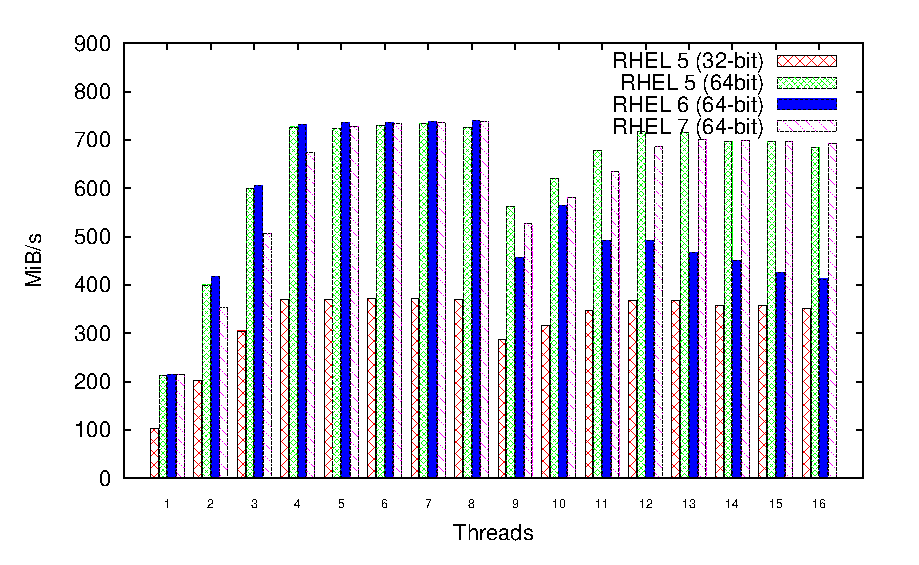
\includegraphics[width=15cm]{fig/tests/difference.eps} % Or .pdf
%\includegraphics[width=10cm,keepaspectratio]{fig/ISK-scheme}
\caption{The~differences between 32 and~64-bit of~RHEL 5 and~RHEL 7 installation.}
\label{fig:testing:difference}
\end{figure}

\par{
The~differences between 64-bit RHELs are much smaller, yet the~RHEL 7 has worse performance when not on a~peak. Furthermore, the~peak speed is the~same, but is reached with one thread more, so it seems that on RHEL 7, the~system is interrupting the~threads more frequently. It can be also by~worse optimization, but this seems to~be less probable, because for a~single thread, the~speed is the~same for all three versions.
}

\par{
Another interesting point is what happens with RHEL 6 after amount of~threads reaches the~limit of~PUs. At first is still close to~other 64 bits systems, but after 10 threads, the~performance is decreasing to~almost half of~RHEL 5 and~7.
}

\par{
In an effort to~find reason of~this difference on RHEL, these tests were done (each of~them was independent and~not affecting the~others):
\begin{itemize}
\item Scheduler settings of~RHEL6 were changed through {\tt sysctl} to~have the~same configuration as on RHEL7.
\item Current versions of~GCC and~OpenMP\footnote{GCC 4.8.2 
with other requested libraries was installed alongside of~the~distribution's 4.4.7 
into a~custom directory. {\tt Makefile} was edited respectively.} %footnote
libraries were manually installed.
\item The~tested application was run also as multiple parallel processes with a~single thread, instead of~one process with multiple threads using GNU {\tt parallel} program.
\end{itemize}
}

\par{
Scheduler settings and~compiler/library versions had just a~small effect 
on the~performance drop on RHEL6. There were just small differences. 
Running the~application as multiple processes with a~single thread, on the~other side, was completely different and~proved even better, than the~results from other systems.
}

\begin{figure}[h!]
  \centering
 \includegraphics[width=15cm]{fig/tests/r6_parallel.eps} % Or .pdf
%\includegraphics[width=10cm,keepaspectratio]{fig/ISK-scheme}
\caption{The~speed of~single thread runs of~RdRand test in dependency of~amount of~parallel runs. Per-process and~total speeds are showed.}
\label{fig:testing:r6parallel}
\end{figure}

\par{
Because changing of~the~GCC and~OpenMP library version did not change the~behavior, nor the~scheduler options, it seems that the~cause is rather in kernel code itself. According of~Jiří Hladký, RHEL 6 has also confirmed similar behavior for other applications that uses more threads: it seems that the~threads are not running concurrently, but sequentially.
}

\par{
This theory was verified by~running time measurement, using {\tt clock()} from {\tt time.h}. Results for 1--16 threads are in \fullref{attachment:times-of-threads-rhel6}. This test measured time for generating in a~single thread and~also total time. This found that up to~8 threads (the~breakpoint) is the~total time the~same as time of~each thread, continually growing. With 9 and~more thread, speed of~a~single thread fall down to~values similar to~4-5 threads, but the~total time goes up to~multiply times of~any of~the~thread. Besides, the~times of~the~threads become more fluctuating. This supports the~theory about sequential ordering of~threads by~kernel, when there are more threads than processing units.
}

\par{
A~possible way how to~remove this performance issue, is to~use a~producent--consument model, where the~generating threads would run independently and~fed a~buffer as fast as they could and~a~single slower thread would not slowdown all application.
}

%..............................................................................
%\newpage
\subsection{Size Dependency}
\begin{tabular}{|l|c|l|}
 \hline
 OS & Arch. & Machine \\
 \hline
  \hline
 RHEL 5 & x86\_64 & \machine{hp-aladdin-01.lab.bos.redhat.com}\\
 \hline
\end{tabular}

\par{
In this test, functions \function{rdrand_get_bytes_retry} and~\function{rdrand_get_uint64_array_retry} were compared in different sizes of~the~memory area that was filled with random numbers. The~goal of~this test was to~find if there is some difference between these two functions; if the~additional logic in the~first one has an measurable impact.
}

\begin{lstlisting}[frame=none, basicstyle=\footnotesize\ttfamily, language=Bash, numbers=none, numberstyle=\tiny\color{black},caption= {Test command for chunk size dependency.}
,label={lst:testing:size}]
./RdRand -r1 -d5 -m METHOD -c SIZE 
\end{lstlisting}


\par{
For a~better visibility, the~figure with measured values is split to~two parts. The~\figref{fig:testing:bytesArrayLow} shows the~difference from 1 to~32 of~64-bit numbers (quadwords) and~\figref{fig:testing:bytesArrayHi} shows the~rest, from 64 to~8192 generated numbers.
}


\begin{figure}[h!]
  \centering
 \includegraphics[width=12cm]{fig/tests/sizeDependency_low.eps} % Or .pdf
%\includegraphics[width=10cm,keepaspectratio]{fig/ISK-scheme}
\caption{The~difference of~two functions on different sizes of~filled memory area, from 1 to~32 quadwords.}
\label{fig:testing:bytesArrayLow}
\end{figure}

\begin{figure}[h!]
  \centering
 \includegraphics[width=12cm]{fig/tests/sizeDependency_hi.eps} % Or .pdf
%\includegraphics[width=10cm,keepaspectratio]{fig/ISK-scheme}
\caption{The~difference of~two functions on different sizes of~filled memory area, from 64 to~8192 quadwords.}
\label{fig:testing:bytesArrayHi}
\end{figure}

\par{
On these figures it is not much apparent, but in numeric data can be found that there is a~very small difference and~the~\function{rdrand_get_bytes_retry} is about 1 \%  slower in the~\figref{fig:testing:bytesArrayLow}. Then the~difference is getting smaller and~at the~size of~8192 quadwords it is just 0.06 \%. 
}

\par{
The~difference is more apparent on small sizes, but as it is not bigger than the~standard deviation, the~\function{rdrand_get_bytes_retry} can be safely used in most times.
}


%..............................................................................
%\pagebreak
\subsection{Fast and~Secure Generating}\label{subsec:testing:fastVsSecure}
\begin{tabular}{|l|c|l|}
 \hline
 OS & Arch. & Machine \\
 \hline
  \hline
 RHEL 5 & x86\_64 & \machine{hp-aladdin-01.lab.bos.redhat.com}\\
  \hline
 RHEL 5 & x86\_64 & \machine{intel-brickland-01.lab.eng.rdu.redhat.com}\\
 \hline
 RHEL 6 & x86\_64 & \machine{hp-aladdin-01.lab.bos.redhat.com}\\
  \hline
 RHEL 7 & x86\_64 & \machine{hp-aladdin-01.lab.bos.redhat.com}\\
 \hline
\end{tabular}

\par{
Because the~secure methods, described in the~section \ref{subsec:api:secure}~\nameref{subsec:api:secure} (both functions \function{rdrand_get_uint64_array_reseed_delay} and~its {\tt \_skip} twin), should not be used in parallel threads\footnote{See \ref{subsec:api:secure}}, only a~single thread comparison between them and~the~\function{rdrand_get_bytes_retry} as a~fast method was made. The~speed was measured on two different machines with different type of~CPUs (Intel Core i7 and~Intel Xeon).
}

\par{
In tables in this section is shown that the~delay method is the~slowest.The~common, fast method is about one thousand times faster than the~skipping method; this is according expectations, because just one per thousand values is used. 
}

\par{
Reason, why on RHEL 5 is the~delay method just 0.008~MiB/s, is unknown, but it seems probable, that it depends on how kernel sleeps and~wakes sleeping processes.
}

\begin{table}[h!]
\begin{center}
\begin{tabular}{|l|c|c|}
  \hline
   & hp-aladdin-01 & intel-brickland-01\\
  \hline
  Fast & 214.530~MiB/s & 73.846~MiB/s\\ 
  \hline
  Delay &  0.008~MiB/s & 0.008~MiB/s\\
  \hline
  Skip & 0.218~MiB/s & 0.074~MiB/s\\
  \hline
\end{tabular}
\caption{Comparison of~speed of~a~fast method of~generating ({\tt rdrand\_get\_bytes\_retry}) and~two variants of~secure generating on RHEL 5 on two machines.}
\label{tab:testing:fastAndSecure1}
\end{center}
\end{table}


\begin{table}[h!]
\begin{center}
\begin{tabular}{|l|c|c|}
  \hline
   & RHEL 6 & RHEL 7\\
  \hline
  Fast & 216.660~MiB/s & 218.347~MiB/s\\ 
  \hline
  Delay &  0.103~MiB/s & 0.101~MiB/s\\
  \hline
  Skip & 0.223~MiB/s & 0.215~MiB/s\\
  \hline
\end{tabular}
\caption{Comparison of~speed of~a~fast method of~generating ({\tt rdrand\_get\_bytes\_retry}) and~two variants of~secure generating on hp-aladdin-01.}
\label{tab:testing:fastAndSecure2}
\end{center}
\end{table}

\par{
The~speed of~the~given by~\function{rdrand_get_uint64_array_reseed_skip} should be possible to~enhance by~using more threads for the~skipping, but implementing of~this functionality directly in the~library would add unwanted dependency for OpenMP (it is used in the~test and~generator application for multithreading, but library itself can be compiled without it). Because of~this, I decided to~do not implement it and~just note it here that if someone would need higher speed, he or she will probably need to~implement its own variant of~the~reseeding function.
}

\par{
Also note, that while the~skipping speed on the~Brickland machine is about one third of~the~Aladdin (see \fullref{subsec:testing:halfPerf} for more about this difference), the~delay is roughly the~same. This is because the~skipping method speed depends on speed of~RdRand per thread, while the~delay method does not.
}

%..............................................................................
%\pagebreak
\subsection{Half performance on some machines}\label{subsec:testing:halfPerf}

\par{All tested machines with an Intel Xeon CPU (the~Brickland, for example) had just half performance of~expected values (and~in comparison with desktop/laptop processors).
}

\par{
We passed this to~Intel Premier program, yet the~only information we received is:
\begin{quote}
The~expectation need to~be set that RDRAND is slower on IVT-EX 
because IVT is missing some optimizations that IVB has 
and~the~measurements ran confirm that after 5 threads, 
the~RdRand throughput maxes out at 375~MiB/s.
\end{quote}
Unfortunately, this is not telling us anything useful and~just it raises more 
questions about security of~this solution, whether the~optimizations can affect not just the~speed.
}

%..............................................................................
%\pagebreak
\subsection{Underflow}
\par{
On \machine{dell-pr1700-02.lab.bos.redhat.com}, when acquiring values from RdRand in more than four threads (no matter whether this library was used, or some other program), the~RdRand wasn't able to~meets the~requirements and~calls of~the~instructions began to~fail. No such another case was found, so it seems to~be just a~flaw on the~specific silicon.
}

%------------------------------------------------------------------------------
\section{Specifications of~Referenced Machines}

\machineDeclare{dell-pr1700-02.lab.bos.redhat.com}{Intel(R) Xeon(R) CPU E3-1285 v3 @ 3.60GHz}{4 GB}{Dell Precision T1700, 4 GB RAM. The~internal RNG was not able to~handle more than four parallel threads at November 2013.}


\machineDeclare{hp-aladdin-01.lab.bos.redhat.com}{Intel(R) Core (TM) i7-3920XM CPU @ 2.90GHz (1 NUMA node, 8 cores, HT\footnote{Hyper-Threading})}{4 GB}{HP elitebook 8770w, used for performance and~statistical tests.}

\machineDeclare{intel-brickland-01.lab.eng.rdu.redhat.com}{ Intel(R) Xeon(R) CPU E7-4890 v2 @ 2.80GHz (4 NUMA nodes, 60 cores, HT)}{128 GB}{Used for performance tests.}

\machineDeclare{intel-brickland-02.lab.eng.rdu.redhat.com}{ Intel(R) Xeon(R) CPU E7-4890 v2 @ 2.80GHz (4 NUMA nodes, 60 cores, HT)}{128 GB}{Used only for statistical tests.}

\machineDeclare{intel-canoepass-01.lab.eng.rdu.redhat.com}{ Intel(R) Xeon(R) CPU E5-2697 v2 @ 2.70GHz (2 NUMA nodes, 24 cores, HT)}{32 GB}{Used only for statistical tests.}

\machineDeclare{intel-canoepass-02.lab.eng.rdu.redhat.com}{ Intel(R) Xeon(R) CPU E5-2697 v2 @ 2.70GHz (2 NUMA nodes, 24 cores, HT)}{32 GB}{Used only for statistical tests.}

%=========================================================================
